\chapter{工欲善其事, 必先利其器}

既然我们准备实现我们宏伟的目标,那么首先我们就需要为实现这个目标做好准备,所谓磨刀不误砍柴工.急急忙忙的开始并不是个好主意.那么我们先来精心挑选自己的工具吧.我们需要准备些什么呢?
\section{一门合适的编程语言}
可以使用的编程语言太多,作者也没有兴趣一一介绍.D2IM的开发使用了C语言.因为在作者眼中C语言是高效而优美的(很多人可能并不这样认为),你也可以使用C++或者JAVA,这是你的自由.
\section{一个高效的编辑器}
作者是VIM的脑残粉,所以作者毫不犹豫的推荐VIM.黑客世界中还有一款极其著名的编辑器叫EMACS,关于VIM和EMACS孰优孰劣,V党和E党常年论战但无定论.作者并不想引起争端,并且作者没有用过EMACS所以不便妄谈,总之最适合你的编辑器便是最好的编辑器.

作者将在下面给出VIM和EMACS的简单安装和配置方法.如果你使用的是其他编辑器,你可以跳过这两个小节,也可以在这两小节中选一种作为入门学习.学会任何一种都会终生受益的,请相信作者.

\subsection{VIM的安装和配置}
VIM是免费软件,官方网站为\textcolor[rgb]{0.0,0.0,1.0}{\uline{\url{http://www.vim.org/}}},你可以在这上面找到它的下载连接。你只需根据自己的系统选择对应的下载即可。
\begin{figure}[htpb]
\centering

\includegraphics[width=1in]{tools/pic/vim_logo.jpg}
\caption{VIM LOGO}
\end{figure}

如果你是windows用户,你可以\href{ftp://ftp.vim.org/pub/vim/pc/gvim73_46.exe}{\textcolor[rgb]{0.0,0.0,1.0}{\uline{点击这里}}}下载VIM在windows下的安装文件,这个链接版本是V73.46,你也可以进入官网下载最新版本。下载完成后安装即可,注意在“Install Options”选项框出现时(如图\ref{fig:vim_install_options}),至少选中下列选项:
\begin{itemize}
\item Vim executables and runtime files
\item Vim console program (vim.exe)
\item Create .bat files for command line use
\item Add an Edit-with-Vim context menu entry
\item Create a \_vimrc if it doesn't exist
\item Create plugin directories in VIM
\end{itemize}

\begin{figure}[htbp]
\centering
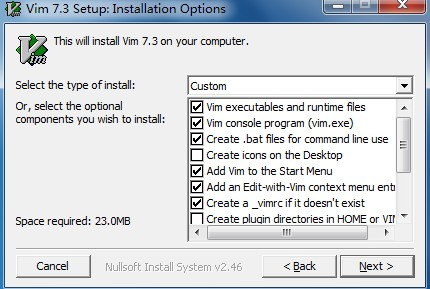
\includegraphics{tools/pic/vim_install_options.jpg}
\caption{VIM安装}
\label{fig:vim_install_options}
\end{figure}

如果你的WINDOWS是中文版,注意去掉Options中的“Native Language Support”,因为这个选项可能导致VIM的提示行显示乱码。

安装完成后会弹出一个VIM README文件,这时候关闭即可,如果你关心你也可以在...找到这个文件。

然后我们尝试安装VIM的中文帮助文档。VIM自带英文文档,如果我们需要我们也可以安装中文文档,这将对英语不好的同学提供很多便利。WINDOWS用户可以\href{ftp://ftp.vim.org/pub/vim/pc/gvim73_46.exe}{\textcolor[rgb]{0.0,0.0,1.0}{\uline{点击这里}}}下载VIMDOC的汉化版。注意在选择VIM所在的安装文件夹时,安装程序尝试寻找vim.exe文件所在的目录,但是如果程序找不到,就需要你为安装程序指定(如图\ref{fig:vimdoc_install_place})。指定VIM所在目录时一定要指定为vim.exe所在目录,否则安装完成后可能VIM找不到中文帮助文件。
\begin{figure}[htbp]
\centering
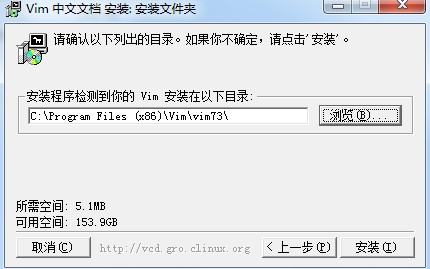
\includegraphics{tools/pic/vimdoc_install_place.jpg}
\caption{VIMDOC安装}
\label{fig:vimdoc_install_place}
\end{figure}

如果你的系统是debian/ubuntu,你可以使用如下命令安装vim到你的系统上:
\begin{lstlisting}
sudo apt-get install vim
\end{lstlisting}

你也可以选择使用源码编译的方式安装vim,这将给你更多为VIM自定义的便利。
\begin{lstlisting}
./configure --with-feature=huge     \
            --prefix=/usr/bin       \
            CFLAGS="-O3 -????"
make
sudo make install
\end{lstlisting}


\begin{lstlisting}

Align
一个对齐的插件,用来排版,面对一堆乱七八糟的代码时,用来对齐代码,功能强大,不过用到
的机会不多
http://www.vim.org/scripts/script.php?script_id=521
Mru
http://www.vim.org/scripts/script.php?script_id=521
给vim增加MRU功能,也就是保留最近打开的文件记录,:MRU打开,q退出,很方便,有过一个支持
菜单的类似的插件
不过对于我这样的不用菜单的用户,还是这个命令行的好用一点,因为经常使用,所以我映射
到了F2
功能强大的代码注释工具,用来注释或者取消注释,支持很多语言,可以对文本块操作,写代码
NERD_comments
功能强大的代码注释工具,用来注释或者取消注释,支持很多语言,可以对文本块操作,写代码
离不了,呵呵
最常用到的快捷键是"c

a.vim
在.c/.h之间切换,写代码必备

bufexplorer.vim
列出当前打开的buffer,可以很容易的切换到和删除选定的buffer,必备插件之一

c.vim
c/c++ support,让你用编写c/c++程序时如虎添翼,有很多贴心的功能,每个功能都有快捷键
,不过一部分和NERD_comments冲突
如果经常编写一些单文件的c程序,但是不想写makefile,用这个,他帮你完成,F9编译并链接,
ctrl-F9运行

calendar.vim
日历插件,有了它,用vim来写日记很方便

csExplorer.vim
color theme浏览插件,列出所有的vim color theme到一个列表中,选中后按回车即可应用相
应的color theme,试验color theme时再也不用一次次输入:colo theme_name了,从上百个
color theme中选择自己喜欢的theme时有用

cscope_maps.vim
cscope的vim插件,提供快捷键操纵cscope,好东东,如果你在用cscope的话

favex.vim
FavEx : Favorite file and directory explorer ,可以添加目录和文件到收藏夹,可以把
经常编辑的文件添加到收藏夹来,在文件打开以后,"ff新增文件到收藏夹,"fd新增目录到
收藏夹

lookupfile.vim
五星级推荐的好插件!我觉得它是vim上最伟大的插件之一,提供多种方式查找文件,让你在复
杂的目?树中也能轻松自如找到你要的文件

matchit.vim
扩展了vim的%功能,让%可以匹配的,不再仅仅是括号,支持多种语言.必备插件之一

parenquote.vim
给选中的文字加上引号,支持( { [ < ' " `,选中后,"加上你想要添加的符号,比如选中abc
后,"(,得到(abc)

snippetEmu.vim
扩展了vim的abbr缩写功能,支持占位符,支持变量替换,强烈推荐

taglist.vim
vim的代码浏览器,生成函数列表,支持跳转,可以根据光标λ置查询到当前的函数名,使用
vim的程序员必备!个人认为是最伟大的插件之一

utl.vim
给vim增加url的识别功能,但是功能远不只是支持url,还有更多,详情见utl的帮助

vcscommand.vim
给vim整合了cvs/subversion功能,不用离开vim环境也能执行常用的cvs/subversion操作了

viki.vim
vim的wiki,没怎么用过,据说很好用,详情可以看滇狐的主页
http://edyfox.codecarver.org/html/viki.html

vis.vim
可以对选中的文本块执行ex操作,尤其是visual block模式下,vim自己是不支持的.选中后,
:B 加上ex命令

visincr.vim
给vim增加生成递增或者递减数列的功能,支持十进制,十六进制,日期,星期等,功能强大灵活

winmanager.vim
给vim增加IDE的功能,提供目录浏览和buffer浏览功能,因为显示器太小,感觉太占空间,所以
单独使用bufexplorer,而且现在vim7的netrw功能也够强大,所以感觉比较鸡肋,而且貌似很
久没有更新,所以基本不用

yankring.vim
类似emacs的king ring,给vim的yank也增加缓冲,vim本身只缓冲删除的字符串,不缓冲yank
的内容
\end{lstlisting}
安装完成后,需要对VIM进行一定的配置。如果是WINDOWS,配置文件在VIM安装目录下(如图),名称为\_vimrc,如果系统为Linux,则VIM配置文件存在于\$HOME文件夹下,名称为.vimrc。打开对应配置文件,删除所有默认配置并加入以下内容:
\begin{lstlisting}
set nocompatible
set number
set wrap
set autoindent
set noswapfile
set cindent
set nobackup
set expandtab
set smartindent
set nowritebackup
set noswapfile

set fileformat  =unix
set tabstop     =4
set shiftwidth  =4
set backspace   =2
set showtabline =0
set mouse       =
set selectmode  =key
set display     =lastline

syntax      on
color       murphy
filetype    plugin on
filetype    indent on

map j               gj
map k               gk
\end{lstlisting}
随着你对VIM的逐渐熟悉,你会继续加入一些自己的设置,上面过的设置只是最基本的。
\subsection{EMACS的安装和配置}
我不会用EMACS,等待有人来补齐这一章.

\subsection{其他编辑器}
我知道的有notepad++和everedit。
\section{选择一款合适的游戏引擎}
D2IM是2.5D游戏,所以我们需要一个合适的2D游戏引擎.作者接触过并使用过的游戏引擎有SDL,HGE和ALLEGRO.我将分别介绍它们.

\subsection{一门合适的脚本语言}
脚本语言是游戏可扩展的重要组成部分.使用最普遍的游戏脚本语言为LUA.

我们将引入自己的脚本语言,我们给它命名为D2S.在本书中,我们将详细的探讨如何构架并实现这个脚本解析引擎.




\section{编译器}
由于D2IM使用了C语言,故必须有一个C语言编译器.我使用的是GCC,你也可以使用微软的编译器.
\subsection{GCC}
我既不是Linux版主, 也不是Linux协会负责人, 我只是一个普普通通的Linux用户. 我做版衫的目的只是想让今年和往年一样, 有一件Linux版衫. 4月5日stephenjy发帖求版衫 , 随即李喵喵投稿, 一片赞同之声之后一个月内无人理睬. 5月15日talentmonkey发帖求版衫, 同样的时间我在Linux协会邮件列表里也求, 一片赞同之声之后继续无人理睬. 之后紧接着boj的每周小聚那天晚上, 我直接跟版主说, 于是版主随手发了个帖子正式征集版衫. 在那之后又过了半个月, 仍然只有李喵喵同学一份投稿. 于是我和李喵喵两个人决定着手开始做版衫, 商量到钱的问题的时候向版主询问建议, 版主的回复是这种细节问题你们自己解.
\subsection{VS2010}
我既不是Linux版主, 也不是Linux协会负责人, 我只是一个普普通通的Linux用户. 我做版衫的目的只是想让今年和往年一样, 有一件Linux版衫. 4月5日stephenjy发帖求版衫 , 随即李喵喵投稿, 一片赞同之声之后一个月内无人理睬. 5月15日talentmonkey发帖求版衫, 同样的时间我在Linux协会邮件列表里也求, 一片赞同之声之后继续无人理睬. 之后紧接着boj的每周小聚那天晚上, 我直接跟版主说, 于是版主随手发了个帖子正式征集版衫. 在那之后又过了半个月, 仍然只有李喵喵同学一份投稿. 于是我和李喵喵两个人决定着手开始做版衫, 商量到钱的问题的时候向版主询问建议, 版主的回复是这种细节问题你们自己解.

\section{选择合适的调试器}
我既不是Linux版主, 也不是Linux协会负责人, 我只是一个普普通通的Linux用户. 我做版衫的目的只是想让今年和往年一样, 有一件Linux版衫. 4月5日stephenjy发帖求版衫 , 随即李喵喵投稿, 一片赞同之声之后一个月内无人理睬. 5月15日talentmonkey发帖求版衫, 同样的时间我在Linux协会邮件列表里也求, 一片赞同之声之后继续无人理睬. 之后紧接着boj的每周小聚那天晚上, 我直接跟版主说, 于是版主随手发了个帖子正式征集版衫. 在那之后又过了半个月, 仍然只有李喵喵同学一份投稿. 于是我和李喵喵两个人决定着手开始做版衫, 商量到钱的问题的时候向版主询问建议, 版主的回复是这种细节问题你们自己解.
\subsection{GDB}
我既不是Linux版主, 也不是Linux协会负责人, 我只是一个普普通通的Linux用户. 我做版衫的目的只是想让今年和往年一样, 有一件Linux版衫. 4月5日stephenjy发帖求版衫 , 随即李喵喵投稿, 一片赞同之声之后一个月内无人理睬. 5月15日talentmonkey发帖求版衫, 同样的时间我在Linux协会邮件列表里也求, 一片赞同之声之后继续无人理睬. 之后紧接着boj的每周小聚那天晚上, 我直接跟版主说, 于是版主随手发了个帖子正式征集版衫. 在那之后又过了半个月, 仍然只有李喵喵同学一份投稿. 于是我和李喵喵两个人决定着手开始做版衫, 商量到钱的问题的时候向版主询问建议, 版主的回复是这种细节问题你们自己解.
\subsection{VS2010}
我既不是Linux版主, 也不是Linux协会负责人, 我只是一个普普通通的Linux用户. 我做版衫的目的只是想让今年和往年一样, 有一件Linux版衫. 4月5日stephenjy发帖求版衫 , 随即李喵喵投稿, 一片赞同之声之后一个月内无人理睬. 5月15日talentmonkey发帖求版衫, 同样的时间我在Linux协会邮件列表里也求, 一片赞同之声之后继续无人理睬. 之后紧接着boj的每周小聚那天晚上, 我直接跟版主说, 于是版主随手发了个帖子正式征集版衫. 在那之后又过了半个月, 仍然只有李喵喵同学一份投稿. 于是我和李喵喵两个人决定着手开始做版衫, 商量到钱的问题的时候向版主询问建议, 版主的回复是这种细节问题你们自己解.

\section{Makefile使用}
我既不是Linux版主, 也不是Linux协会负责人, 我只是一个普普通通的Linux用户. 我做版衫的目的只是想让今年和往年一样, 有一件Linux版衫. 4月5日stephenjy发帖求版衫 , 随即李喵喵投稿, 一片赞同之声之后一个月内无人理睬. 5月15日talentmonkey发帖求版衫, 同样的时间我在Linux协会邮件列表里也求, 一片赞同之声之后继续无人理睬. 之后紧接着boj的每周小聚那天晚上, 我直接跟版主说, 于是版主随手发了个帖子正式征集版衫. 在那之后又过了半个月, 仍然只有李喵喵同学一份投稿. 于是我和李喵喵两个人决定着手开始做版衫, 商量到钱的问题的时候向版主询问建议, 版主的回复是这种细节问题你们自己解.

\section{如何管理你的代码}
推荐使用SVN/GIT管理你的代码.共享你的源代码吧
我既不是Linux版主, 也不是Linux协会负责人, 我只是一个普普通通的Linux用户. 我做版衫的目的只是想让今年和往年一样, 有一件Linux版衫. 4月5日stephenjy发帖求版衫 , 随即李喵喵投稿, 一片赞同之声之后一个月内无人理睬. 5月15日talentmonkey发帖求版衫, 同样的时间我在Linux协会邮件列表里也求, 一片赞同之声之后继续无人理睬. 之后紧接着boj的每周小聚那天晚上, 我直接跟版主说, 于是版主随手发了个帖子正式征集版衫. 在那之后又过了半个月, 仍然只有李喵喵同学一份投稿. 于是我和李喵喵两个人决定着手开始做版衫, 商量到钱的问题的时候向版主询问建议, 版主的回复是这种细节问题你们自己解.
